\documentclass[tikz]{standalone}
\makeatletter
\tikzset{lls/.code=\tikz@addtransform{\pgflowlevelsynccm}}
\newcommand*\tikzbeginlowlevelscope[1]{\pgfextra{\pgfsyssoftpath@addtocurrentpath\pgfsys@beginscope\pgflowlevel{\tikzset{#1}}}}
\newcommand*\tikzendlowlevelscope{\pgfextra{\pgfsyssoftpath@addtocurrentpath\pgfsys@endscope}}
\makeatother
\begin{document}
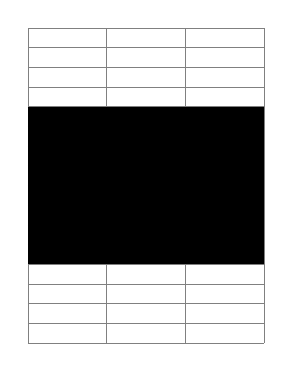
\begin{tikzpicture}
\draw[help lines, ystep=2.5mm] (0,-2) grid (3,2);
\draw[line width=5mm] (0,0) -- ++(right:1)
  \tikzbeginlowlevelscope{yscale=2}
    -- ++(right:1)
    \tikzbeginlowlevelscope{yscale=2}
      -- ++(right:1)
    \tikzendlowlevelscope
  \tikzendlowlevelscope
;
\end{tikzpicture}
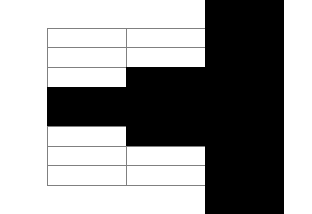
\begin{tikzpicture}
\draw[help lines, ystep=2.5mm] (0,-1) grid (3,1);
\draw[line width=5mm]                (0,0) -- ++(right:1);
\draw[line width=5mm][yscale=2, lls] (1,0) -- ++(right:1);
\draw[line width=5mm][yscale=4, lls] (2,0) -- ++(right:1);
\end{tikzpicture}
\end{document}
